\documentclass[11pt,a4paper]{article}
\usepackage[spanish,es-nodecimaldot]{babel}	% Utilizar español
\usepackage[utf8]{inputenc}					% Caracteres UTF-8
\usepackage{graphicx}						% Imagenes
\usepackage[hidelinks]{hyperref}			% Poner enlaces sin marcarlos en rojo
\usepackage{fancyhdr}						% Modificar encabezados y pies de pagina
\usepackage{float}							% Insertar figuras
\usepackage[textwidth=390pt]{geometry}		% Anchura de la pagina
\usepackage[nottoc]{tocbibind}				% Referencias (no incluir num pagina indice en Indice)
\usepackage{enumitem}						% Permitir enumerate con distintos simbolos
\usepackage[T1]{fontenc}					% Usar textsc en sections
\usepackage{amsmath, yhmath}						% Símbolos matemáticos
\usepackage{subcaption}

% Comando para poner el nombre de la asignatura
\newcommand{\asignatura}{Simulación de Sistemas}
\newcommand{\autor}{Vladislav Nikolov Vasilev}
\newcommand{\titulo}{Práctica 3}
\newcommand{\subtitulo}{Modelos de Simulación Dinámicos y Discretos}

% Configuracion de encabezados y pies de pagina
\pagestyle{fancy}
\lhead{\autor{}}
\rhead{\asignatura{}}
\lfoot{Grado en Ingeniería Informática}
\cfoot{}
\rfoot{\thepage}
\renewcommand{\headrulewidth}{0.4pt}		% Linea cabeza de pagina
\renewcommand{\footrulewidth}{0.4pt}		% Linea pie de pagina

\begin{document}
\pagenumbering{gobble}

% Pagina de titulo
\begin{titlepage}

\begin{minipage}{\textwidth}

\centering


\includegraphics[scale=0.5]{img/ugr.png}\\

\textsc{\Large \asignatura{}\\[0.2cm]}
\textsc{GRADO EN INGENIERÍA INFORMÁTICA}\\[1cm]

\noindent\rule[-1ex]{\textwidth}{1pt}\\[1.5ex]
\textsc{{\Huge \titulo\\[0.5ex]}}
\textsc{{\Large \subtitulo\\}}
\noindent\rule[-1ex]{\textwidth}{2pt}\\[3.5ex]

\end{minipage}

\vspace{0.5cm}

\begin{minipage}{\textwidth}

\centering

\textbf{Autor}\\ {\autor{}}\\[2.5ex]
\textbf{Rama}\\ {Computación y Sistemas Inteligentes}\\[2.5ex]
\vspace{0.3cm}


\includegraphics[scale=0.3]{img/etsiit.jpeg}

\vspace{0.7cm}
\textsc{Escuela Técnica Superior de Ingenierías Informática y de Telecomunicación}\\
\vspace{1cm}
\textsc{Curso 2019-2020}
\end{minipage}
\end{titlepage}

\pagenumbering{arabic}
\tableofcontents
\thispagestyle{empty}				% No usar estilo en la pagina de indice

\newpage

\setlength{\parskip}{1em}

\section{\textsc{Mi segundo modelo de simulación discreto}}

En esta sección vamos a estudiar primero el comportamiento de un modelo de
simulación de un servidor con una única cola, y después de $m$ servidores
con una única cola. Vamos a ver cómo distintos métodos de incremento del
itempo pueden afectar al funcionamiento del sistema, y discutiremos cuál
de ellos es mejor.

\subsection{Método de incremento fijo del tiempo}

El primer método de incremento del tiempo que vamos a estudiar es el incremento
fijo. Como su propio nombre indica, el tiempo se va incrementando en una cantidad
fija, tal como lo hace un reloj normal. Esta cantidad viene decidida por la persona
que va a utilizar el sistema (pueden ser minutos, segundos, milésimas, horas, etc.).

Debido a la naturaleza de dicho incremento, la variable de tiempo debe ser tratada
como una variable entera. Por tanto, aunque en el pesudocódigo proporcionado se
generen las llegadas y el servicio utilizando valores reales, dichos valores obtenidos
deben ser transformados a enteros, redondeándolos al entero más próximo. Además, si
el valor que se obtiene al hacer las transformaciones correspondientes es 0, se
debe devolver 1, ya que si no, se generaría un suceso en el tiempo actual y, al
incrementar el tiempo en una unidad, ese suceso se quedaría en un tiempo anterior
al nuevo actual, y por tanto, nunca se podría llevar a cabo.

Una vez dicho esto, vamos a experimentar con el sistema. Para ello, vamos a utilizar
las siguientes unidades de tiempo: horas, medias horas, cuartos de hora, minutos, segundos,
décimas de segundo y milésimas de segundo. En cada caso simularemos que se tienen que
atender 10000 clientes, y repetiremos cada ejecución 100 veces. De ahí, podremos
ver los valores obtenidos en cada simulación y los valores medios para el número
medio de clientes en la cola y el porcentaje de tiempo de ocio del servidor. Además,
veremos cuánto tarda cada simulación y el tiempo medio que han tardado todas las simulaciones,
aunque en la tabla se reflejará solo este último valor. Vamos a pintar también en algunos de los
casos gráficas para ver cómo van evolucionando los resultados que se obtienen en cada una de las
100 simulaciones, para ver si de verdad se parecen a los resuldatos medios. Los valores de
\texttt{tlleg} y \texttt{tserv} son 9 y 6 minutos, respectivamente, aunque aparecerán reflejados
según la unidad de tiempo correspondiente.

Una vez hechas todas las simulaciones, se han obtenido los siguientes resultados:

\begin{table}[H]
\resizebox{\textwidth}{!}{%
\begin{tabular}{|c|c|c|c|c|}
\hline
\texttt{tlleg} & \texttt{tserv} & \textbf{\begin{tabular}[c]{@{}c@{}}Num. medio\\ clientes cola\end{tabular}} & \textbf{\begin{tabular}[c]{@{}c@{}}\% medio tiempo\\ ocio servidor\end{tabular}} & \textbf{\begin{tabular}[c]{@{}c@{}}Tiempo ejecución\\ medio\end{tabular}} \\ \hline
0.15 & 0.1 & 0.0262607 & 0.138175 & 0.000593755 \\ \hline
0.3 & 0.2 & 0.21363 & 2.93386 & 0.000889945 \\ \hline
0.6 & 0.4 & 0.550758 & 11.669 & 0.000932894 \\ \hline
9 & 6 & 1.25962 & 31.5821 & 0.00104538 \\ \hline
540 & 360 & 1.33738 & 33.3778 & 0.0119809 \\ \hline
5400 & 3600 & 1.32336 & 33.4474 & 0.134477 \\ \hline
54000 & 36000 & 1.344 & 33.1509 & 1.33758 \\ \hline
\end{tabular}%
}
\caption{Resultados obtenidos por el incremento de tiempo fijo.}
\label{tab:fijo}
\end{table}

A primera vista podemos ver que a medida que \texttt{tlleg} y \texttt{tserv}
usan unidades más pequeñas de tiempo (y por tanto, sus valores son más altos),
los resultados obtenidos se van incrementando, hasta el punto en el que parece
que se estabilizan. Lo que sucede es que cuando las unidades de tiempo son grandes,
los valores de \texttt{tlleg} y \texttt{tserv} son menores que 0. Al llamar a
los generadores, se producirán valores próximos a 0, y al redondearlos, estos pasan
a valer 0. Como el generador no puede devolver 0, devuelve 1. Por tanto, lo que
estamos haciendo en realidad es sobreestimar la duración de un suceso, por lo que
los valores obtenidos no serán reales, ya que se va acumulando el error al haber
sobreestimado. Este es un problema de los métodos de incremento fijo del tiempo, y
a la vez es una fuerte desventaja, ya que dependiendo de la unidad de tiempo que se
utilice, los valores obtenidos serán más o menos representativos de los que se podrían
obtener de forma teórica.

Aparte de esto, si analizamos los resultados vemos que los tiempos medios de ejecución
se van incrementando, debido a que se debe incrementar más veces el reloj hasta
llegar a un suceso. El valor medio del número medio de clientes en cola, $Q(n)$, parece
estabilizarse en torno a 1.33, y el valor medio del porcentaje de tiempo de ocio
del servidor, $PTO(n)$ parece estabilizarse al final en torno al 33\%. Para unidades
de tiempo superiores a los segundos los resultados obtenidos no son representativos,
ya que se quedan demasiado lejos de los valores obtenidos al utilizar unidades
de tiempo más pequeñas. Por tanto, parece ser que, en caso de utilizar generadores
de incremento fijo, lo suyo sería utilizar unidades de tiempo más pequeñas (es decir,
que los valores sean grandes), ya que de esta forma se cometerá menos error.

Ahora, pasemos a estudiar el comportamiento del sistema para cada simulación.
Vamos a ver qué resultados se han obtenido para el número de medio de clientes
en cola y para el porcentaje de tiempo de ocio del servidor. Vamos a estudiar
dicha evolución con gráficas, tal y como se mencionó anteriormente, para ver
si hay mucha discrepancia entre los valores medios obtenidos. Vamos a realizar
un estudio de todos los resultados de forma conjunta.

A continuación se pueden ver las gráficas mencionadas en el párrafo anterior:

\begin{figure}[H]
	\centering
	\begin{subfigure}{.5\textwidth}
		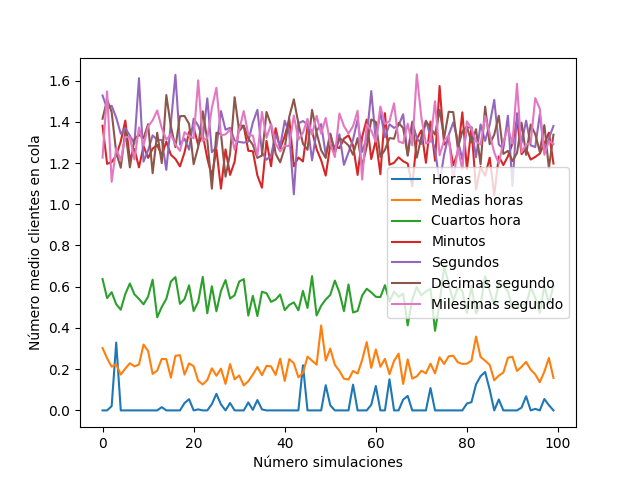
\includegraphics[scale=0.44]{img/fijo-q}
		\subcaption{Número medio de clientes en la cola.}
		\label{fig:fijo-q}
	\end{subfigure}%
	~
	\begin{subfigure}{.5\textwidth}
		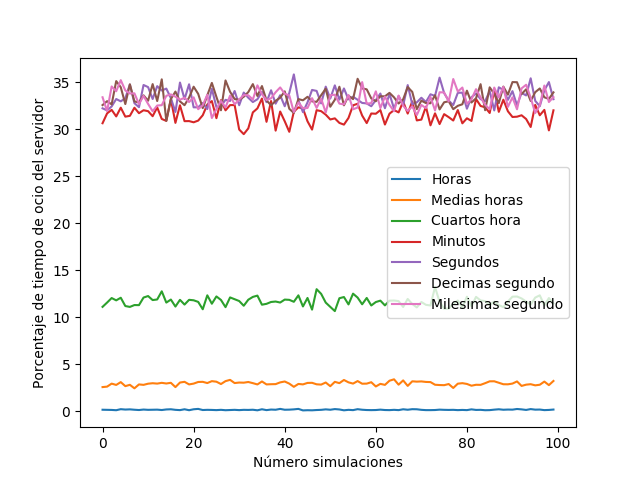
\includegraphics[scale=0.44]{img/fijo-pto}
		\subcaption{Porcentaje de tiempo de ocio del servidor.}
		\label{fig:fijo-pto}
	\end{subfigure}

	\caption{Variación de los resultados a lo largo de las simulaciones.}
	\label{fig:fijo}
\end{figure}

Vemos que, tal y como habíamos dicho antes, para unidades de tiempo más grandes
que los minutos, los valores de $Q(n)$ y $PTO(n)$ están bastante alejados del resto.
En aquellos casos en los que se usa como unidad de tiempo una que es el minuto
o inferior a ésta los resultados sí que están próximos, y parece que se aproximan
a los valores medios obtenidos. Vemos que en todos los casos existe cierta variabilidad
entre los resultados de una simulación o de otra. Por tanto, no podríamos fiarnos solo
de los resultados obtenidos por una simulación, sino que, tal y como llevamos haciendo
hasta ahora, habría que hacer algunas simulaciones y promediar.

Por tanto, como pequeña conclusión de esta parte, podemos sacar que es importante
escoger una unidad de tiempo adecuada, ya que si no lo es, va a provocar que
los resultados no sean del todo buenos. Si hemos escogido una unidad de
tiempo adecuada, los resultados que obtengamos serán buenos, ya que estarán bastante
relacionados entre sí, justo como ha pasado aquí.

\subsection{Método de incremento variable del tiempo}

El siguiente método de incremento del tiempo que vamos a estudiar es el incremento
variable. En este caso, el tiempo no se va incrementando de manera fija como sucedía
anteriormente, si no que se incrementa hasta el suceso más próximo de una. Por
tanto, este método parece ser mucho más eficiente, ya que evita tener que pegar demasiados
saltos y evita errores como los que se producían anteriormente.

Para ver como funciona este tipo de incremento, vamos a realizar los mismos experimentos
que en la sección anterior, de forma que tengamos resultados comparables. A continuación
se puede ver una tabla con los resultados:

\begin{table}[H]
\resizebox{\textwidth}{!}{%
\begin{tabular}{|c|c|c|c|c|}
\hline
\texttt{tlleg} & \texttt{tserv} & \textbf{\begin{tabular}[c]{@{}c@{}}Num. medio\\ clientes cola\end{tabular}} & \textbf{\begin{tabular}[c]{@{}c@{}}\% medio tiempo\\ ocio servidor\end{tabular}} & \textbf{\begin{tabular}[c]{@{}c@{}}Tiempo ejecución\\ medio\end{tabular}} \\ \hline
0.15 & 0.1 & 1.32894 & 33.3767 & 0.000731009 \\ \hline
0.3 & 0.2 & 1.32033 & 33.4927 & 0.000986358 \\ \hline
0.6 & 0.4 & 1.335 & 33.3979 & 0.000692968 \\ \hline
9 & 6 & 1.32356 & 33.5117 & 0.000969834 \\ \hline
540 & 360 & 1.35058 & 33.1523 & 0.000713056 \\ \hline
5400 & 3600 & 1.33727 & 33.3192 & 0.000690027 \\ \hline
54000 & 36000 & 1.34364 & 33.2906 & 0.000895026 \\ \hline
\end{tabular}%
}
\caption{Resultados obtenidos por el incremento de tiempo variable.}
\label{tab:var}
\end{table}

Podemos ver que en general los resultados obtenidos en todos los casos son más
o menos iguales, tanto para los valores de $Q(n)$ como de $PTO(n)$. Además, los
tiempos de ejecución son casi los mismos en todos los casos, por lo tanto son
independiendes de la unidad de tiempo utilizada, a diferencia del caso anterior.
Aquí los tiempos son casi constantes, ya que existe poca o muy poca variación entre
éstos. Observando los tiempos de la tabla \ref{tab:fijo}, vemos que, a medida
que usamos medidas de tiempo más pequeñas, los tiempos medios se van haciendo más grandes,
experimentando lo que parece ser un crecimiento lineal, ya que el número de veces
que se incrementará el reloj aumenta. Aquí, los incrementos solo dependen del
número de sucesos, mientras que en el caso anterior dependían de la unidad de
medida de tiempo. Por tanto, de aquí podemos concluir que, efectivamente, el
incremento variable del tiempo es muchísimo más eficiente que el incremento
fijo del tiempo, ya que el primero es constante, independientemente de la unidad
de medida utilizada, mientras que el segundo es lineal, ya que en función de la unidad
de medida del tiempo utilizada tardará más o menos (será más rápido para las unidades
más grandes).

Si comparamos la calidad de los resultados, vemos también que en general son mucho
mejores. Vemos que incluso utilizando unidades de tiempo grandes, como por ejemplo
horas, los valores medios obtenidos son muy parecidos a los que se obtienen
con unidades más pequeñas, como por ejemplo las décimas de segundo. Esto es
completamente lo opuesto a lo que sucedió anteriormente, ya que los resultados
eran muy dispares. Por tanto, parece que el incremento de tiempo variable
es independiente de la unidad de medida usada, a diferencia del incremento
fijo del tiempo.

Si observamos los resultados obtenidos en cada una de las simulaciones, nos
encontramos con lo siguiente:

\begin{figure}[H]
	\centering
	\begin{subfigure}{.5\textwidth}
		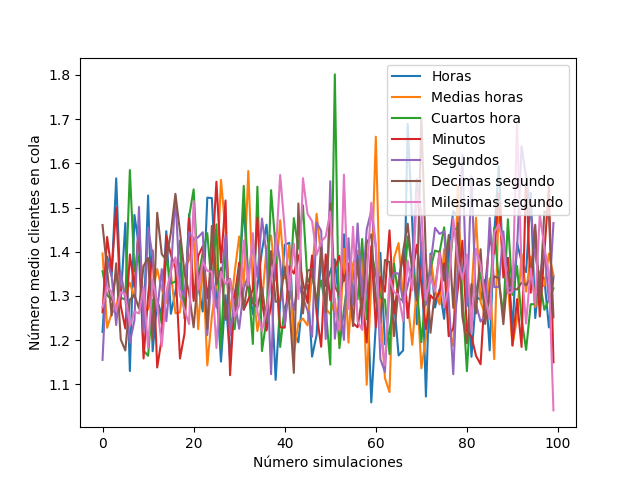
\includegraphics[scale=0.44]{img/var-q}
		\subcaption{Número medio de clientes en la cola.}
		\label{fig:var-q}
	\end{subfigure}%
	~
	\begin{subfigure}{.5\textwidth}
		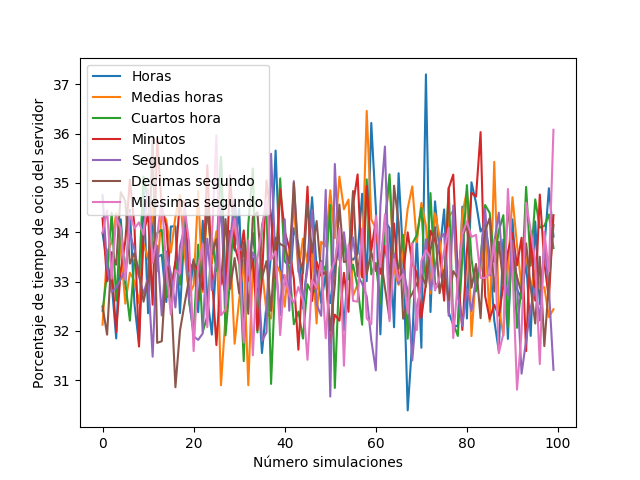
\includegraphics[scale=0.44]{img/var-pto}
		\subcaption{Porcentaje de tiempo de ocio del servidor.}
		\label{fig:var-pto}
	\end{subfigure}

	\caption{Variación de los resultados a lo largo de las simulaciones.}
	\label{fig:var}
\end{figure}

Tal y como pasaba antes, vemos que existen variaciones entre los resultados
obtenidos para cada simulación. No obstante, vemos que son bastante
parecidos en general. Parece que oscilan en torno a la media, tal y
como pasaba antes. De nuevo, si hubiésemos tomado el resultado de una única
simulación como el correcto, nos hubiésemos equivocado ya que, tal y como
hemos visto, existe una ligera variación en los resultados.

Ahora que hemos visto los dos modelos, podemos hacer una comparación de
cómo de buenos son los resultados ofrecidos. Para ello, nos podemos
servir de las expresiones teóricas. Para hacer los cálculos, vamos a utilizar
los tiempos expresados en minutos, para facilitar el cómputo. Primero
tenemos que calcular $\rho$:

\begin{equation}
	\rho = \frac{\texttt{tserv}}{\texttt{tlleg}} = \frac{6}{9} =
	\frac{2}{3} = 0.\wideparen{6}
\end{equation}

Ahora, podemos calcular el valor teórico de $Q(n)$:

\begin{equation}
	Q(n) = \frac{\rho^2}{1-\rho} = \frac{\big(\frac{2}{3}\big)^2}{1 - \frac{2}{3}} =
	\frac{\frac{4}{9}}{\frac{1}{3}} = \frac{12}{9} = \frac{4}{3} = 1.\wideparen{3}
\end{equation}

Y también el de $PTO(n)$:

\begin{equation}
	PTO(n) = 100 \cdot (1 - \rho) = 100 \cdot \Big(1 - \frac{2}{3}\Big) 
	100 \cdot \frac{1}{3} = \frac{100}{3} = 33.\wideparen{3}
\end{equation}

Si comparamos los resultados de la tabla \ref{tab:fijo} con los teóricos,
vemos que el incremento fijo de tiempo solo ofrece resultados parecidos
a los teóricos cuando las unidades de tiempo utilizadas son pequeñas.
A partir de los segundos podríamos decir realmente que son resultados correctos.
A excepción de los minutos, que ofrecen unos resultados aproximados aunque
con cierto error, las medidas de tiempo más grandes nos ofrecerían valores
con demasiado error como para considerarlos válidos.

En cambio, todos los resultados medios obtenidos por el incremento variable
del tiempo, tal y como se pueden ver en la tabla \ref{tab:var}, son muy próximos,
por no decir casi iguales, a los resultados teóricos, independientemente de
la unidad de medida del tiempo utilizada. Por tanto, la calidad de los resultados
ofrece el incremento variable del tiempo es muy superior a la del incremento fijo
del tiempo.

Como conclusión, podemos decir que, tras estudiar los dos casos, hemos visto
que el incremento variable del tiempo es órdenes de magnitud más eficiente
que el incremento fijo del tiempo, y además, permite obtener unos resultados
de mayor calidad, independientemente de qué medida del tiempo se use.

\subsection{Modelo dinámico discreto de $m$ servidores con una única cola}

En esta sección vamos a estudiar un modelo algo más complejo que el anterior,
en el cuál tenemos $m$ servidores con una única cola.

\end{document}

